\documentclass[11pt]{article}
\usepackage[margin=1in]{geometry}
\usepackage{amsmath,amssymb}
\usepackage{booktabs}
\usepackage{graphicx}
\usepackage{hyperref}
\usepackage{xcolor}
\title{\bf Railway Timetabling Benchmark Lab:\\ Size-Ladder Report (B0--B6 + P1)}
\author{ASU Trans+AI Lab \\ \small repo: \texttt{asu-trans-ai-lab/railway-timetabling-lab} --- \texttt{benchmark\_lab/}}
\date{\today}

\begin{document}
\maketitle

\begin{abstract}
We report the first complete run of the classical railway scheduling laboratory over a size ladder of
single-track (C1) corridor instances plus a double-track (C2) probe. The solver ladder comprises B0
priority heuristics, B1 Lagrangian relaxation, B2 time-indexed MILP (HiGHS), B3 LR-based
branch-and-bound, B4 CP-SAT (OR-Tools), B5 individual-path column generation with exact pricing, B6
branch-and-price with departure-window branching, and P1 group-supercolumn CG. All methods emit one
common reporting record; every bound is validity-checked against generator ground truth. Headlines:
the exact-equivalence gate passes with three independent exact solvers agreeing on every proven
instance; the individual-path LP shows a real 18.1\% integrality gap that a full-component group
supercolumn closes to zero; branch-and-price closes the same gap by branching; instances with
8--12 trains remain open with certified intervals. Two claims made earlier in development were
retracted when convergence checks failed --- the retractions are part of this report.
\end{abstract}

\section{Instances and ground truth}
Feasible-first generation (infrastructure $\to$ serial-schedule incumbent $\to$ free-flow intended
arrivals $\to$ release compression), manifest-recorded. Objective: $\sum_k |\mathrm{arr}_k -
\mathrm{intended}_k|$; unit capacity per (link, minute) cell with 3-min headway; dwell only on sidings.

\begin{table}[h]\centering\small
\caption{The size ladder. Proven optima certified by $\geq$2 independent exact solvers.}
\begin{tabular}{lccll}
\toprule
instance & trains & serial UB & ground truth & status \\
\midrule
toy\_native & 3 & --- & \textbf{12} & proven (MILP=B\&B=CP-SAT=B\&P) \\
C1\_L4\_n4\_seed1 & 4 & 75 & \textbf{29} & proven (4 solvers) \\
C1\_L4\_n4\_seed2 & 4 & 71 & \textbf{20} & proven (4 solvers) \\
C1\_L6\_n6\_seed3 & 6 & 276 & \textbf{57} & proven (CP-SAT 0.7s; LR-B\&B incumbent agrees) \\
C1\_L8\_n8\_seed11 & 8 & 678 & $[\mathbf{105},\,\mathbf{138}]$ & OPEN \\
C1\_L10\_n10\_seed12 & 10 & 1375 & $[106,\,189]$ & OPEN \\
C1\_L12\_n12\_seed13 & 12 & 2446 & $[155,\,388]$ & OPEN \\
C2\_L6\_n8\_seed21 (double track) & 8 & 544 & $[39,\,43]$ & open (120 s probe) \\
\bottomrule
\end{tabular}
\end{table}

\section{Proven tier: method comparison}
\begin{table}[h]\centering\small
\caption{Exact tier. UB = returned objective; proven = optimality certificate. B2 is a documented
RESTRICTED model (toward-destination arcs, departure pad, dwell cap): UB-only, no LB claim.}
\begin{tabular}{llrrlr}
\toprule
instance & method & UB & LB & proven & time (s) \\
\midrule
toy & B0 (any rule) & 12 & --- & no & 0.1 \\
toy & B2 MILP & 12 & --- & (restricted) & 0.0 \\
toy & B4 CP-SAT & 12 & 12 & yes & 0.0 \\
toy & B5 CG & 12 & 12.00 & LP tight & 0.0 \\
toy & B6 B\&P & 12 & 12 & yes (root) & 0.0 \\
\midrule
seed1 & B0 best (class) & 29 & --- & no & 0.4 \\
seed1 & B2 MILP & 29 & --- & (restricted) & 4.6 \\
seed1 & B3 LR-B\&B & 29 & 29 & yes (1385 nodes) & 55.7 \\
seed1 & B4 CP-SAT & 29 & 29 & yes & 0.0 \\
seed1 & B5 CG & 42 & \textbf{23.75} & LP converged & 4.5 \\
seed1 & B6 B\&P & 29 & 29 & \textbf{yes (185 nodes)} & 115.8 \\
\midrule
seed2 & B4 CP-SAT & 20 & 20 & yes & 0.0 \\
seed2 & B5 CG / B6 B\&P & 20 & 20.00 & LP tight / root & 3--4 \\
\midrule
seed3 & B0 best (rand5) & 75 & --- & no & 3.9 \\
seed3 & B2 MILP & 63 & --- & (restriction binds!) & 38.0 \\
seed3 & B4 CP-SAT & 57 & 57 & yes & 0.7 \\
seed3 & B5 CG & 69 & 51.00 & LP converged & 9.0 \\
seed3 & B6 B\&P & 57 & 51.00 & no (budget) & 150.9 \\
\bottomrule
\end{tabular}
\end{table}

Observations. (i) CP-SAT is the fastest exact solver throughout. (ii) On seed3, B2's dwell cap
($s_{\max}=15$) binds: its restricted optimum 63 exceeds the true optimum 57 --- visible only because
the restriction is labeled UB-only. (iii) The LR-based B\&B (B3) proves seed1 but on seed3 its
Lagrangian bound stalls (36.3 after 6441 nodes) while its incumbent finds the optimum: LR bound
weakness quantified per instance (LR 36.3 $<$ path-LP 51 $<$ opt 57).

\section{The convexification result (P1)}
\begin{center}
\begin{tabular}{lccc}
\toprule
relaxation (seed1) & LP value & integrality gap & cost \\
\midrule
individual paths (B5, exact pricing, converged) & 23.75 & 18.1\% & 4.5 s \\
group supercolumns, component split $[1,3]$ & 25.25 & 12.9\% & 4.5 s \\
\textbf{full 4-train component as one group} & \textbf{29.00 = integer = optimum} & \textbf{0\%} & 114.7 s \\
\bottomrule
\end{tabular}
\end{center}
Making the strong interaction primal-visible inside one jointly-feasible column removes the
integrality gap entirely (single column, one pricing round); the group-size cost (24 order
enumerations) is the $K_{\max}$ trade-off. \emph{Label:} the pricer is order-enumeration, not full
joint DP, so LP values are \emph{restricted} group LPs; the certified-true-group-LP claim awaits the
designed pair joint DP (PLAN \S5b). On seed3, split $[3,3]$ groups add essentially nothing
(restricted group LP $\to$ 51.17 vs individual 51): \textbf{component-covering groups are what matter}.

\section{Open tier and retractions}
For $n\in\{8,10,12\}$ no method proves optimality in budget. Certified intervals come from CP-SAT
UBs and, for $n=8$, a \emph{converged} B\&P root LP (105 $>$ CP-SAT's 102). Two development-time
claims were retracted by convergence checks and are recorded in the ledger: (a) three B\&P node
bounds on the open tier (node CG iteration-capped $\Rightarrow$ not valid bounds); (b) the seed3
``75\% gap closed'' group-LP reading (an unconverged restricted value, 55.50, that fell to 51.17
under deeper pricing). Restricted-master values are meaningful only at pricing convergence.

\section{Topology probe (C2)}
Eight trains on the same corridor length: single track $[105,138]$ vs double track $[39,43]$ ---
the interaction-density lever the C2/CM experiment family will sweep.

\section{Timetable views (seed1, proven optimum)}
\begin{center}
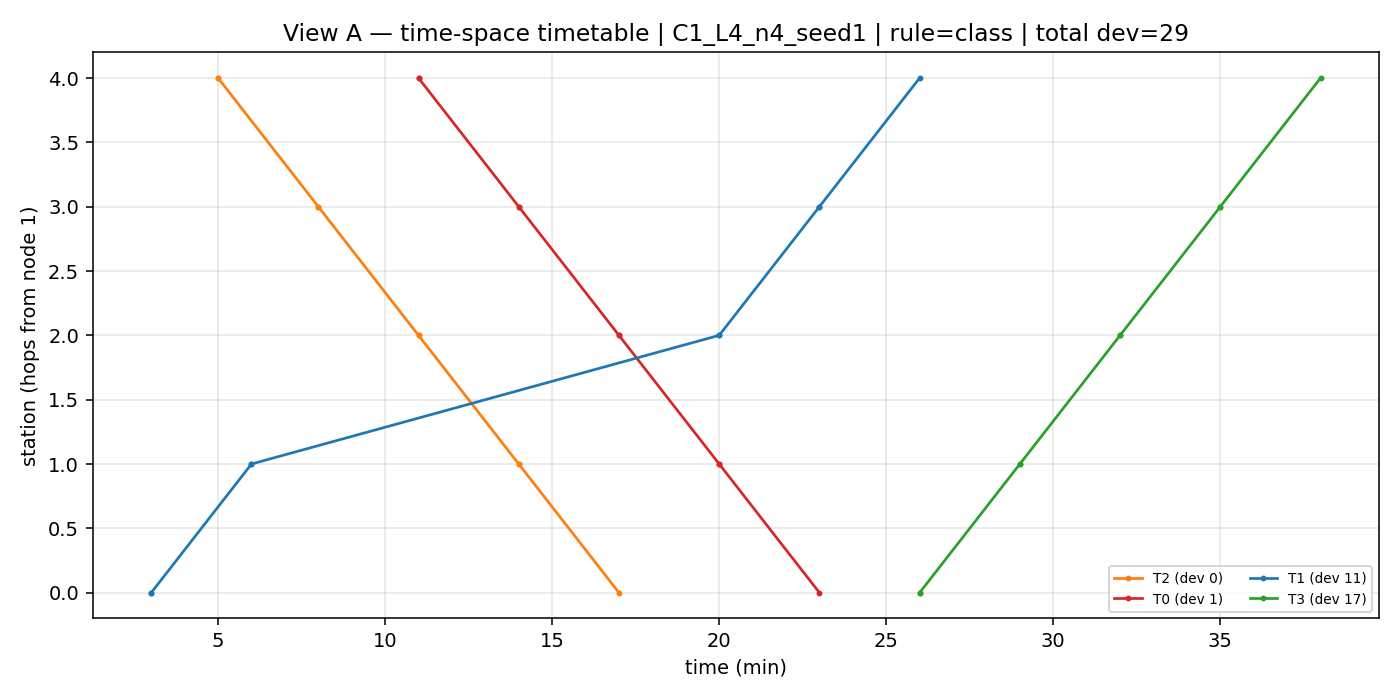
\includegraphics[width=.95\textwidth]{C1_L4_n4_seed1_viewA.png}\\[4pt]
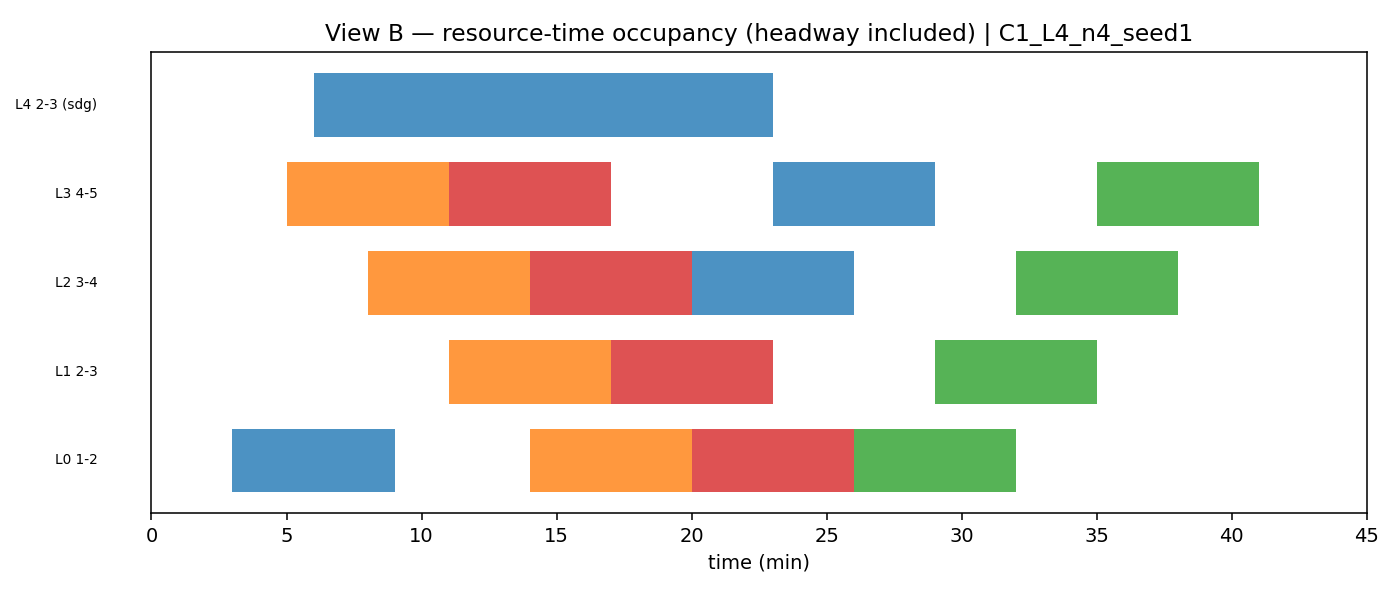
\includegraphics[width=.95\textwidth]{C1_L4_n4_seed1_viewB.png}
\end{center}

\section*{Reproducibility}
\texttt{benchmark\_lab/run\_pipeline.py} regenerates \texttt{pipeline\_records.csv};
\texttt{make\_report.py} rebuilds the markdown ledger; every instance carries a
\texttt{manifest.json} with seed, serial schedule, and ground truth. Common record schema:
\texttt{record\_schema.py}.

\end{document}
